\chapter{Hamilton-Jacobi Theory}

% 2017/04/18
\section{Hamilton-Jacobi: Relating HJB to PMP}
Recall the HJB theorem: $u^*$ is the global minimizer to
\begin{gather}
  \int_0^T L(x,u)\dif t + \Psi(x(T))
\end{gather}
s.t.\ $\dot x=f(x,u)$ if it solves
\begin{align}
  & -\pder{J^*}{t} = \min_u \left\{ L(x,u) + \pder{J^*}{x} f(x,u) \right\} \label{eq:hjb} \\
  & J^*(x,T) = \Psi(x)
\end{align}
where $J^*(x,t)$ is the optimal cost-to-go from $t$ to $T$ starting at $x$.

Note that the term within the curly brackets on the right-hand side of \eqref{eq:hjb} is a Hamiltonian:
\begin{gather}
  H(x,u,\lambda) = L(x,u) + \lambda\trans f(x,u)
\end{gather}
with the odd choice of $\lambda=\partial J^*{}\trans(x,t)/\partial x$.

From Pontryagin, $u^*=\min_u H(x,u,\lambda)$ (locally). However, the minimization in \eqref{eq:hjb} is global. What if we insisted on a global minimizer $u^*$?

\begin{defi}
  The Hamiltonian $H(x,u,\lambda)$ is \emph{regular} if, for every $x,\lambda$, there is a unique global minimizer $u^*(x,\lambda)$, i.e.\
  \begin{gather}
    H(x,u^*(x,\lambda),\lambda) < H(x,u,\lambda) \quad \forall u\neq u^*(x,\lambda).
  \end{gather}
\end{defi}

From HJB, we know that we should pick $\lambda=\partial J^*{}\trans(x,t)/\partial x$. Assuming $H$ is regular, we should use
\begin{gather}
  u^*\left(x,\pder{J^*{}\trans}{x}\right).
\end{gather}
PMP states we should find $\lambda$ from
\begin{align}
  & \dot \lambda = -\pder{H\trans}{x}, \\
  & \lambda(T) = \pder{\Psi}{x}(x(T)).
\end{align}
Hamilton-Jacobi (HJ) states we should get our new ``costate'' $\partial J^*/\partial x$ from a ``modified'' HJB:
\begin{gather}
  \min_u \left\{ L(x,u) + \pder{J^*}{x} f(x,u) \right\} = \min_u \left\{ H\left(x,u,\pder{J^*{}\trans}{x}\right) \right\} = H\Bigg( x, u^*\left(x,\pder{J^*{}\trans}{x}\right), \pder{J^*{}\trans}{x} \Bigg).
\end{gather}
HJ is preferable to HJB because it makes statements about $u^*$ (directly) rather than $J^*$.

\begin{thm}[Hamilton-Jacobi]
  If $H$ is regular and $J^*(x,t)$ satisfies the HJ equation
  \begin{gather}
    \begin{dcases}
      -\pder{J^*}{t} = H\Bigg( x, u^*\left(x,\pder{J^*{}\trans}{x}\right), \pder{J^*{}\trans}{x} \Bigg) \\
      J^*(x,T) = \Psi(x)
    \end{dcases}
  \end{gather}
  then
  \begin{gather}
    u^*\left(x,\pder{J^*{}\trans}{x}\right).
  \end{gather}
  is the global optimal solution.
\end{thm}

\paragraph{Example} \mbox{}
\begin{align}
  \min_u {} & \int_0^1 2u^2(t)\dif t + (x(1)-1)^2 \\
  \text{s.t. } & \dot x = u,\quad x,u\in\R
\end{align}
This is almost LQ except for the wrong terminal condition.
\begin{align}
  H &= 2u^2 + \lambda u \\
  \pder{H}{u} &= 4u + \lambda \\
  \pder{^2 H}{u^2} &= 4 > 0,
\end{align}
so $H$ is strictly convex in $u$, and $H$ is regular. By HJ,
\begin{align}
  u^*(x,\lambda) = -\frac{\lambda}{4}
\end{align}
Replace $\lambda$ with $\partial J^*/\partial x$ and plug into the HJ equation:
\begin{align}
  -\pder{J^*}{t} &= H\Bigg( x, u^*\left(x,\pder{J^*{}\trans}{x}\right), \pder{J^*{}\trans}{x} \Bigg) \\
                 &= 2 \underbrace{\left( -\frac{\partial J^*/\partial x}{4} \right)^2}_{u^2} + \underbrace{\pder{J^*}{x}}_{\lambda} \cdot \underbrace{\left( -\frac{\partial J^*/\partial x}{4} \right)}_{u} \\
                 &= \frac{(\partial J^*/\partial x)^2}{8} - \frac{(\partial J^*/\partial x)^2}{4} = -\frac{1}{8} \left(\pder{J^*}{x}\right)^2 \\
  \pder{J^*}{t} &= \frac{1}{8} \left(\pder{J^*}{x}\right)^2 \\
  J^*(x,1) &= (x-1)^2
\end{align}
What is $J^*(x,t)$? A standard trick is to assume separability, i.e.\
\begin{gather}
  J^*(x,t) = F_1(x) F_2(t).
\end{gather}
Then,
\begin{gather}
  F_1(x) F_2'(t) = \frac{1}{8} [F_1'(x) F_2(t)]^2 = \frac{1}{8} [F_1'(x)]^2 F_2^2(t).
\end{gather}
We have $[F_1'(x)]^2\sim F_1(x)$, so $F_1(x)$ is probably quadratic in $x$. We also have $F_2'(t)\sim F_2^2(t)$, so $F_2(t)$ is probably $\sim 1/t$. Let's try
\begin{align}
  J^*(x,t) &= \frac{ax^2 + bx + c}{\alpha t + \beta}. \\
  \shortintertext{Then,}
  \pder{J^*}{x} &= \frac{2ax + b}{\alpha t + \beta} \\
  \left(\pder{J^*}{x}\right)^2 &= \frac{4a^2x^2 + 4abx + b^2}{(\alpha t + \beta)^2} \\
  \pder{J^*}{t} &= -\alpha \frac{ax^2 + bx + c}{(\alpha t + \beta)^2}
\end{align}
The HJ equation is then
\begin{align}
  0 &= \pder{J^*}{t} - \frac{1}{8} \left(\pder{J^*}{x}\right)^2 \\
    &= \frac{-\alpha(ax^2 + bx + c)}{(\alpha t + \beta)^2} - \frac{1}{8} \frac{4a^2x^2 + 4abx + b^2}{(\alpha t + \beta)^2} \\
    &= \bigg(\alpha a + \frac12 a^2\bigg) x^2 + \bigg(\alpha b + \frac12 ab\bigg) x + \bigg(\alpha c + \frac18 b^2\bigg)
\end{align}
This gives us two equations and five unknowns:
\begin{alignat}{2}
  x^2:\ & \alpha a + \frac12 a^2 = 0 & \qquad & \alpha = -\frac12 a \quad \text{(or $a=0$)} \\
  x^1:\ & \alpha b + \frac12 ab = 0 && \alpha = -\frac12 a \quad \text{(or $b=0$)} \\
  x^0:\ & \alpha c + \frac18 b^2 = 0
\end{alignat}
We also need to consider the boundary conditions:
\begin{gather}
  J^*(x,1) = (x-1)^2 \\
  \frac{ax^2 + bx + c}{\alpha + \beta} = x^2 - 2x + 1 \\
  \begin{aligned}
    x^2:\ & \frac{a}{\alpha+\beta} = 1 \\
    x^1:\ & \frac{b}{\alpha+\beta} = -2 \\
    x^0:\ & \frac{c}{\alpha+\beta} = 1
  \end{aligned}
\end{gather}
This gives us three additional equations, making for five equations and five unknowns. The solution is
\begin{gather}
  \begin{dcases}
    a = 2 \\
    b = -4 \\
    c = 2 \\
    \alpha = -1 \\
    \beta = 3
  \end{dcases} \\
  J^*(x,t) = \frac{2x^2 - 4x + 2}{-t + 3} = 2 \frac{(x-1)^2}{3-t} \\
  u^* = -\frac{\partial J^*/\partial x}{4} \\
  \boxed{u^* = \frac{1-x}{3-t}}
\end{gather}
This is the globally optimal solution!

This problem could have been solved by turning it into an LQ problem. We need to turn the terminal cost from $(x(1)-1)^2$ into $\hat x(1)^2$. Let $\hat x=x-1$, so $\dot{\hat x}=\dot x=u$. Then, the problem becomes
\begin{align}
  \min_u {} & \int_0^1 2u^2\dif t + \hat x^2(1) \\
  \text{s.t. } & \dot{\hat x}=u \\
            & \hat x(0) = x_0 - 1
\end{align}
The optimal controller is
\begin{gather}
  u = -R^{-1} B\trans P \hat x = -\frac12 (x-1) p(t),
\end{gather}
where
\begin{align}
  \dot p &= -A\trans P - PA - Q + PBR^{-1}B\trans P \\
  \dot p &= \frac{p^2}{2} \\
  p(1) &= 1
\end{align}

% 2017/04/20
\section{The Tracking Problem}
Given a linear system
\begin{align}
  \dot x &= Ax + Bu, \quad x\in\R^n,u\in\R^m \\
  y &= Cx, \quad y\in\R^p
\end{align}
We would like $y(t)=Cx(t)$ to track a reference trajectory $\mu(t)$.
\begin{center}
  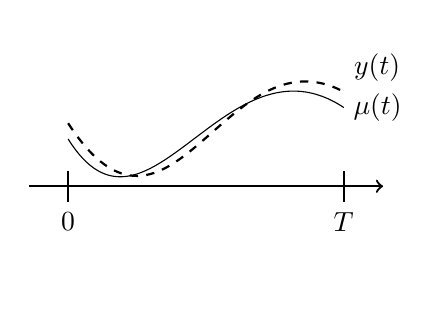
\begin{tikzpicture}
    \draw [->,thick] (-0.5,0) -- (4,0);
    \draw [thick] (0,0.2) -- (0,-0.2) node [below] {$0$};
    \draw [thick] (3.5,0.2) -- (3.5,-0.2) node [below] {$T$};
    \draw (0,0.6) .. controls (1,-1) and (2,2) .. (3.5,1) node [right] {$\mu(t)$};
    \draw [thick,dashed] (0,0.8) .. controls (1.3,-1.2)  and (2,2) .. (3.5,1.2) node [above right] {$y(t)$};
  \end{tikzpicture}
\end{center}
Let the cost be
\begin{gather}
  \min_u \frac12 \int_0^T \Big[ (y-\mu)\trans Q (y-\mu) + u\trans Ru \Big]\dif t + \frac12 \big(y(T)-\mu(T)\big)\trans S \big(y(T)-\mu(T)\big),
\end{gather}
where $Q=Q\trans \succeq 0$, $R=R\trans \succ 0$, and $S=S\trans \succeq 0$. This looks like a LQ problem, but it is not. (\textbf{Check:} To be a LQ problem, the $B$ matrix needs to be invertible.)

This is a ``classical'' control problem. This can be solved using the HJ equation. Typically, it is difficult to solve the PDE, so instead we will verify a claimed solution.

We claim the optimal solution is
\begin{gather}
  u(t) = -R^{-1}B\trans [P(t)x(t) + w(t)],
\end{gather}
where $P(t)$ solves the Riccati equation
\begin{align}
  \dot P &= -A\trans P - PA - C\trans Q C + PBR^{-1}B\trans P \\
  P(T) &= C\trans SC
\end{align}
and $w(t)$ satisfies
\begin{align}
  \dot w &= -(A-BR^{-1}B\trans P)\trans w + C\trans Q \mu \\
  w(T) &= -C\trans S \mu(T)
\end{align}
The optimal cost-to-go is given as
\begin{gather}
  J^*(x,t) = \frac12 x\trans P(t) x + w\trans(t) x + v(t)
\end{gather}
where
\begin{align}
  \dot v &= \frac12 (w\trans BR^{-1}B\trans w - \mu\trans Q\mu) \\
  v(T) &= \frac12 \mu\trans(T) S \mu(T)
\end{align}
Let's verify if the claim is correct using the HJ theorem. Step 1 is to check that the Hamiltonian is regular:
\begin{gather}
  H = \frac12 \Big[ (Cx-\mu)\trans Q(Cx-\mu) + u\trans Ru \Big] + \lambda\trans (Ax + Bu) \\
  \pder{H}{u} = u\trans R + \lambda\trans B = 0 \\
  \boxed{u^* = -R^{-1}B\trans\lambda} \\
  \pder{^2 H}{u^2} = R \succ 0,
\end{gather}
so $u^*$ is a unique global minimizer ($H$ is regular). Step 2 is to substitute $\lambda\trans=\partial J^*/\partial x$:
\begin{gather}
  \pder{J^*}{x} = x\trans P + w\trans \\
  \lambda = Px + w \\
  u^* = -R^{-1} B\trans (Px + w),
\end{gather}
which matches the claim. Step 3 is to show that this choice of $J^*$ satisfies the theorem. We need to check both the boundary condition and the differential equation. For the boundary condition,
\begin{align}
  J^*(x,T) &= \frac12 x\trans P(T) x + w\trans (T) x + v(T) \\
           &= \frac12 x\trans C\trans SCx - \mu\trans(T) SCx + \frac12 \mu\trans(T) S\mu(T) \\
           &= \frac12 x\trans C\trans SCx - \frac12 \mu\trans(T) SCx - \frac12 x\trans C\trans S\mu(T) + \frac12 \mu\trans(T) S\mu(T) \\
           &= \frac12 (Cx-\mu)\trans S (Cx-\mu) = \Psi(x),
\end{align}
which matches the claim. For the PDE,
\begin{gather}
  -\pder{J^*}{t} = H\bigg( x, u^*\Big(x,\pder{J^*{}\trans}{x}\Big), \pder{J^*{}\trans}{x} \bigg) \\
  \begin{aligned}
    \pder{J^*}{t} &= \frac12 x\trans \dot P x + \dot w\trans x + \dot v \\
    &= \frac12 x\trans \Big( -A\trans P - PA - C\trans Q C + PBR^{-1}B\trans P \Big) x \\
    & \qquad {} - w\trans \Big( A - BR^{-1}B\trans P \Big) x + \mu\trans QCx + \frac12 \Big( w\trans BR^{-1}B\trans w - \mu\trans Q\mu \Big) \\
  \end{aligned} \\
  \begin{aligned}
    -\pder{J^*}{t} &= \frac12 x\trans \Big( A\trans P + PA + C\trans Q C - PBR^{-1}B\trans P \Big) x \\
    & \qquad {} + w\trans \Big( A - BR^{-1}B\trans P \Big) x - \mu\trans QCx - \frac12 \Big( w\trans BR^{-1}B\trans w - \mu\trans Q\mu \Big) \\
  \end{aligned} \label{eq:dJdt_ex}
\end{gather}
The Hamiltonian is
\begin{align}
  H(x,u,\lambda) &= \frac12 (Cx-\mu)\trans Q(Cx-\mu) + \frac12 u\trans Ru + \lambda\trans (Ax + Bu) \\
                 &= \frac12 x\trans C\trans QCx - \mu\trans QCx + \frac12 \mu\trans Q\mu + \frac12 \big(w\trans + x\trans P\big) BR^{-1}RR^{-1}B\trans \big(Px + w\big) \\
                 & \qquad {} + \big(w\trans + x\trans P\big) \big( Ax - BR^{-1}B\trans (Px + w)\big) \\
  \intertext{Expanding and simplifying the last two terms,}
  H(x,u,\lambda) &= \frac12 x\trans C\trans QCx - \mu\trans QCx + \frac12 \mu\trans Q\mu - \frac12 w\trans BR^{-1}B\trans w \\
                 & \qquad {} - \frac12 x\trans PBR^{-1}B\trans Px + w\trans Ax + \underbrace{x\trans PAx}_{\mathclap{(x\trans PAx + x\trans A\trans Px)/2}} - x\trans PBR^{-1}Bw \\
                 &= \frac12 x\trans \Big( C\trans QC + PA + A\trans P - PBR^{-1}B\trans P \Big) x \\
                 & \qquad {} w\trans \Big( A - BR^{-1}B\trans P \Big) x - \mu\trans QCx + \frac12 \mu\trans Q\mu - \frac12 w\trans BR^{-1}B\trans w,
\end{align}
which matches \eqref{eq:dJdt_ex}, as desired.

\paragraph{Example} Self-driving car---lane changes

\begin{center}
  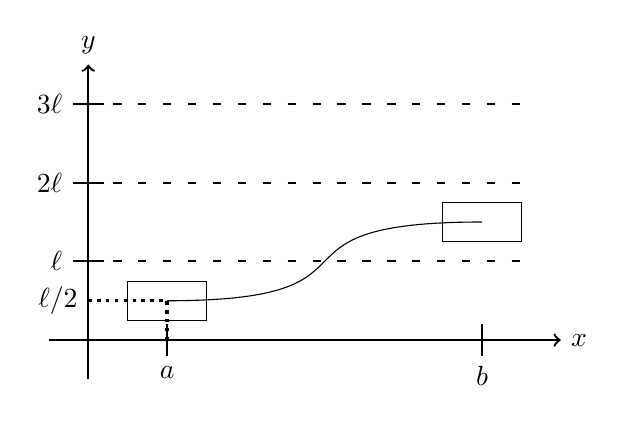
\begin{tikzpicture}
    \draw [->,thick] (-0.5,0) -- (6,0) node [right] {$x$};
    \draw [->,thick] (0,-0.5) -- (0,3.5) node [above] {$y$};
    \draw [thick] (1,0.2) -- ++(0,-0.4) node [below] {$a$};
    \draw [thick] (5,0.2) -- ++(0,-0.4) node [below] {$b$};
    \draw [thick] (0.2,1) -- ++(-0.4,0) node [left] {$\ell$};
    \draw [thick] (0.2,2) -- ++(-0.4,0) node [left] {$2\ell$};
    \draw [thick] (0.2,3) -- ++(-0.4,0) node [left] {$3\ell$};
    \foreach \y in {1,2,3}
    \draw [thick,loosely dashed] (0,\y) -- (5.5,\y);
    \draw (0.5,0.25) rectangle +(1,0.5);
    \draw (4.5,1.25) rectangle +(1,0.5);
    \draw [dotted,very thick] (1,0) -- (1,0.5);
    \draw [dotted,very thick] (0,0.5) node [left] {$\ell/2$} -- (1,0.5);
    \draw (1,0.5) .. controls (4,0.5) and (2,1.5) .. (5,1.5);
  \end{tikzpicture}
\end{center}
Let the state of the system be
\begin{gather}
  x = \begin{bmatrix}
    p_x \\ p_y \\ v_x \\ v_y
  \end{bmatrix}.
\end{gather}
With input $[u_x,u_y]\trans$, the dynamics are
\begin{align}
  \begin{bmatrix}
    \dot p_x \\ \dot p_y \\ \dot v_x \\ \dot v_y
  \end{bmatrix} &= \begin{bmatrix}
    0 & 0 & 1 & 0 \\
    0 & 0 & 0 & 1 \\
    0 & 0 & 0 & 0 \\
    0 & 0 & 0 & 0
  \end{bmatrix} \begin{bmatrix}
    p_x \\ p_y \\ v_x \\ v_y
  \end{bmatrix} + \begin{bmatrix}
    0 & 0 \\
    0 & 0 \\
    1 & 0 \\
    0 & 1
  \end{bmatrix} \begin{bmatrix}
    u_x \\ u_y
  \end{bmatrix} \\
  \begin{bmatrix}
    y_{p_x} \\ y_{p_y}
  \end{bmatrix} &= \begin{bmatrix}
    1 & 0 & 0 & 0 \\
    0 & 1 & 0 & 0
  \end{bmatrix} \begin{bmatrix}
    p_x \\ p_y \\ v_x \\ v_y
  \end{bmatrix}
\end{align}
On T-Square, the Matlab file \texttt{self\_driving\_car.m} is posted.

%%% Local Variables:
%%% mode: latex
%%% TeX-master: "../notes"
%%% End: